\documentclass[multi=page, border=0.1cm]{standalone}
\usepackage{xcolor}
\usepackage{tikz}

\usetikzlibrary{arrows, arrows.meta}
\tikzset{
    larrow/.style={ % style that just defines the arrow tip
        >={Triangle[left,length=6pt,width=4pt]},
        shorten >= 1pt, shorten <= 1pt,
        semithick,
        ->
    }
}

\begin{document}
\begin{page}
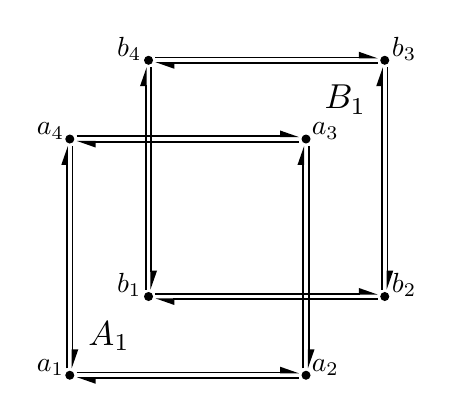
\begin{tikzpicture}
    \tikzstyle{node1}=[draw,shape=circle,color=black,fill=black, scale=0.3]
    \tikzstyle{node2}=[color=black,fill=white]

    \node[node1,label={[xshift=-0.7em, yshift=-0.5em, scale=1] $a_1$}] (a1) at (0,0)   {};
    \node[node1,label={[xshift= 0.7em, yshift=-0.5em, scale=1] $a_2$}] (a2) at (3,0)   {};
    \node[node1,label={[xshift= 0.7em, yshift=-0.5em, scale=1] $a_3$}] (a3) at (3,3)   {};
    \node[node1,label={[xshift=-0.7em, yshift=-0.5em, scale=1] $a_4$}] (a4) at (0,3)   {};
    \node[node1,label={[xshift=-0.7em, yshift=-0.5em, scale=1] $b_1$}] (b1) at (1,1)   {};
    \node[node1,label={[xshift= 0.7em, yshift=-0.5em, scale=1] $b_2$}] (b2) at (4,1)   {};
    \node[node1,label={[xshift= 0.7em, yshift=-0.5em, scale=1] $b_3$}] (b3) at (4,4)   {};
    \node[node1,label={[xshift=-0.7em, yshift=-0.5em, scale=1] $b_4$}] (b4) at (1,4)   {};


     \draw[larrow, transform canvas={yshift= 1pt}] (a1) -- (a2);
     \draw[larrow, transform canvas={yshift=-1pt}] (a2) -- (a1);
     \draw[larrow, transform canvas={xshift=-1pt}] (a2) -- (a3);
     \draw[larrow, transform canvas={xshift= 1pt}] (a3) -- (a2);
     \draw[larrow, transform canvas={yshift=-1pt}] (a3) -- (a4);
     \draw[larrow, transform canvas={yshift= 1pt}] (a4) -- (a3);
     \draw[larrow, transform canvas={xshift= 1pt}] (a4) -- (a1);
     \draw[larrow, transform canvas={xshift=-1pt}] (a1) -- (a4);

     \draw[larrow, transform canvas={yshift= 1pt}] (b1) -- (b2);
     \draw[larrow, transform canvas={yshift=-1pt}] (b2) -- (b1);
     \draw[larrow, transform canvas={xshift=-1pt}] (b2) -- (b3);
     \draw[larrow, transform canvas={xshift= 1pt}] (b3) -- (b2);
     \draw[larrow, transform canvas={yshift=-1pt}] (b3) -- (b4);
     \draw[larrow, transform canvas={yshift= 1pt}] (b4) -- (b3);
     \draw[larrow, transform canvas={xshift= 1pt}] (b4) -- (b1);
     \draw[larrow, transform canvas={xshift=-1pt}] (b1) -- (b4);

    \node[scale=1.25] at (0.5, 0.5) {$A_1$};
    \node[scale=1.25] at (3.5, 3.5) {$B_1$};
\end{tikzpicture}
\end{page}

\begin{page}
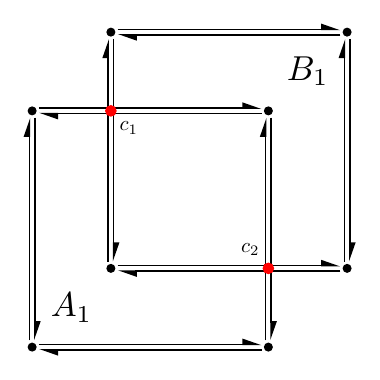
\begin{tikzpicture}
    \tikzstyle{node1}=[draw,shape=circle,color=black,fill=black, scale=0.3]
    \tikzstyle{node2}=[draw,shape=circle,color=red,fill=red, scale=0.4]

    \node[node1] (a1) at (0,0)   {};
    \node[node1] (a2) at (3,0)   {};
    \node[node1] (a3) at (3,3)   {};
    \node[node1] (a4) at (0,3)   {};
    \node[node1] (b1) at (1,1)   {};
    \node[node1] (b2) at (4,1)   {};
    \node[node1] (b3) at (4,4)   {};
    \node[node1] (b4) at (1,4)   {};

     \draw[larrow, transform canvas={yshift= 1pt}] (a1) -- (a2);
     \draw[larrow, transform canvas={yshift=-1pt}] (a2) -- (a1);
     \draw[larrow, transform canvas={xshift=-1pt}] (a2) -- (a3);
     \draw[larrow, transform canvas={xshift= 1pt}] (a3) -- (a2);
     \draw[larrow, transform canvas={yshift=-1pt}] (a3) -- (a4);
     \draw[larrow, transform canvas={yshift= 1pt}] (a4) -- (a3);
     \draw[larrow, transform canvas={xshift= 1pt}] (a4) -- (a1);
     \draw[larrow, transform canvas={xshift=-1pt}] (a1) -- (a4);

     \draw[larrow, transform canvas={yshift= 1pt}]  (b1) -- (b2);
     \draw[larrow, transform canvas={yshift=-1pt}] (b2) -- (b1);
     \draw[larrow, transform canvas={xshift=-1pt}] (b2) -- (b3);
     \draw[larrow, transform canvas={xshift= 1pt}]  (b3) -- (b2);
     \draw[larrow, transform canvas={yshift=-1pt}] (b3) -- (b4);
     \draw[larrow, transform canvas={yshift= 1pt}]  (b4) -- (b3);
     \draw[larrow, transform canvas={xshift= 1pt}]  (b4) -- (b1);
     \draw[larrow, transform canvas={xshift=-1pt}] (b1) -- (b4);

    \node[node2,label={[xshift=0.65em, yshift=-1.3em, scale=0.75] $c_1$}] (c1) at (1,3)   {};
    \node[node2,label={[xshift=-0.65em, yshift=0em, scale=0.75] $c_2$}] (c2) at (3,1)   {};

    \node[scale=1.25] at (0.5, 0.5) {$A_1$};
    \node[scale=1.25] at (3.5, 3.5) {$B_1$};
\end{tikzpicture}
\end{page}

\begin{page}
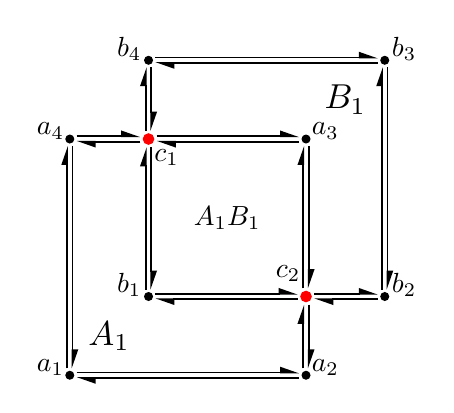
\begin{tikzpicture}
    \tikzstyle{node1}=[draw,shape=circle,color=black,fill=black, scale=0.3]
    \tikzstyle{node2}=[draw,shape=circle,color=red,fill=red, scale=0.4]

    \node[node1,label={[xshift=-0.7em, yshift=-0.5em, scale=1] $a_1$}] (a1) at (0,0)   {};
    \node[node1,label={[xshift= 0.7em, yshift=-0.5em, scale=1] $a_2$}] (a2) at (3,0)   {};
    \node[node1,label={[xshift= 0.7em, yshift=-0.5em, scale=1] $a_3$}] (a3) at (3,3)   {};
    \node[node1,label={[xshift=-0.7em, yshift=-0.5em, scale=1] $a_4$}] (a4) at (0,3)   {};
    \node[node1,label={[xshift=-0.7em, yshift=-0.5em, scale=1] $b_1$}] (b1) at (1,1)   {};
    \node[node1,label={[xshift= 0.7em, yshift=-0.5em, scale=1] $b_2$}] (b2) at (4,1)   {};
    \node[node1,label={[xshift= 0.7em, yshift=-0.5em, scale=1] $b_3$}] (b3) at (4,4)   {};
    \node[node1,label={[xshift=-0.7em, yshift=-0.5em, scale=1] $b_4$}] (b4) at (1,4)   {};

    \node[node2,label={[xshift=0.65em, yshift=-1.5em, scale=1] $c_1$}] (c1) at (1,3)   {};
    \node[node2,label={[xshift=-0.65em, yshift=0em,    scale=1] $c_2$}] (c2) at (3,1)   {};

    \draw[larrow, transform canvas={yshift= 1pt}] (a1) -- (a2);
    \draw[larrow, transform canvas={yshift=-1pt}] (a2) -- (a1);
    \draw[larrow, transform canvas={xshift=-1pt}] (a2) -- (c2);
     \draw[larrow, transform canvas={xshift= 1pt}] (c2) -- (a2);
     \draw[larrow, transform canvas={yshift=-1pt}] (c1) -- (a4);
     \draw[larrow, transform canvas={yshift= 1pt}] (a4) -- (c1);
     \draw[larrow, transform canvas={xshift= 1pt}] (a4) -- (a1);
     \draw[larrow, transform canvas={xshift=-1pt}] (a1) -- (a4);

     \draw[larrow, transform canvas={yshift= 1pt}] (c2) -- (b2);
     \draw[larrow, transform canvas={yshift=-1pt}] (b2) -- (c2);
     \draw[larrow, transform canvas={xshift=-1pt}] (b2) -- (b3);
     \draw[larrow, transform canvas={xshift= 1pt}] (b3) -- (b2);
     \draw[larrow, transform canvas={yshift=-1pt}] (b3) -- (b4);
     \draw[larrow, transform canvas={yshift= 1pt}] (b4) -- (b3);
     \draw[larrow, transform canvas={xshift= 1pt}] (b4) -- (c1);
     \draw[larrow, transform canvas={xshift=-1pt}] (c1) -- (b4);

     \draw[larrow, transform canvas={yshift= 1pt}] (b1) -- (c2);
     \draw[larrow, transform canvas={yshift=-1pt}] (c2) -- (b1);
     \draw[larrow, transform canvas={xshift=-1pt}] (c2) -- (a3);
     \draw[larrow, transform canvas={xshift= 1pt}] (a3) -- (c2);
     \draw[larrow, transform canvas={yshift=-1pt}] (a3) -- (c1);
     \draw[larrow, transform canvas={yshift= 1pt}] (c1) -- (a3);
     \draw[larrow, transform canvas={xshift= 1pt}] (c1) -- (b1);
     \draw[larrow, transform canvas={xshift=-1pt}] (b1) -- (c1);

    \node[scale=1.25] at (0.5, 0.5) {$A_1$};
    \node[scale=1.25] at (3.5, 3.5) {$B_1$};
    \node[scale=1] at (2, 2)  {$A_1B_1$};

\end{tikzpicture}
\end{page}

\end{document}
